\documentclass[11pt]{article}
\usepackage[a4paper,margin=2.2cm]{geometry}
\usepackage[T1]{fontenc}
\usepackage{lmodern}
\usepackage{pgfplots}\pgfplotsset{compat=1.18}
\usepackage{booktabs,array,xcolor,titlesec,fancyhdr,enumitem,caption,tabularx}
\usepackage{microtype}
\usepackage[backend=bibtex,style=numeric-comp,sorting=none,maxnames=3]{biblatex}
\addbibresource{refs.bib}
\definecolor{teal0}{RGB}{0,128,128}
\definecolor{burnt}{RGB}{204,85,0}
\definecolor{ink}{RGB}{38,42,46}
\definecolor{paper}{RGB}{250,249,246}
\definecolor{grayln}{RGB}{200,200,200}
\definecolor{softgreen}{RGB}{46,139,87}
\pagecolor{paper}\color{ink}
\captionsetup{font=small,labelfont={bf,color=teal0}}
\titleformat{\section}{\Large\bfseries\color{teal0}}{\thesection}{0.6em}{}
\titleformat{\subsection}{\large\bfseries\color{burnt}}{\thesubsection}{0.5em}{}
\pagestyle{fancy}\fancyhf{}\renewcommand{\headrulewidth}{0.3pt}
\lhead{\small\color{teal0}Ontology-Grounded Local Inference Eval}\rhead{\small\color{teal0}DreamLab AI \textbullet\ 2026-06-17}
\cfoot{\small\thepage}
\pgfplotsset{
  every axis/.append style={font=\small,axis line style={grayln},tick style={grayln},
    grid=major,major grid style={grayln!40},label style={color=ink},tick label style={color=ink}},
  augstyle/.style={fill=teal0,draw=teal0!60},
  ctlstyle/.style={fill=burnt,draw=burnt!60},
  localstyle/.style={fill=softgreen,draw=softgreen!60},
}
\begin{document}

% =============================================================================
% TITLE PAGE
% =============================================================================
\begin{titlepage}
\centering\vspace*{1.6cm}
{\color{teal0}\Huge\bfseries Can a Local Model Beat\\[4pt] the Frontier?\par}
\vspace{0.6cm}
{\large Ontology-Grounded DiffusionGemma vs.\ Bare Cloud Models\\[2pt]
A KG-as-Oracle A/B Evaluation\par}
\vspace{0.3cm}
{\color{burnt}\large PRD-020 / ADR-112 \textbullet\ 672 isolated runs \textbullet\ 7 models\par}
\vspace{1.2cm}
\begin{tabular}{rl}
\toprule
\textbf{Local + ontology (DiffusionGemma AUG)} & \textbf{0.505} \\
\midrule
Opus 4.8 bare & 0.350 \\
Sonnet 4.6 bare & 0.373 \\
Haiku 4.5 bare & 0.250 \\
Gemini 3.5 Flash bare & 0.423 \\
Gemini 2.5 Flash Lite bare & 0.384 \\
Z.AI (GLM-4.6) bare & 0.342 \\
\midrule
\textbf{\color{burnt}Local model beats every frontier bare} & \color{burnt}\checkmark \\
\bottomrule
\end{tabular}
\vfill
{\small Knowledge graph: Oxigraph/Whelk, 7{,}445 OWL classes (re-indexed June 2026).\\
Ground truth derived from the KG itself. DiffusionGemma 26B-A4B runs on a single local GPU.\par}
\vspace{0.6cm}
{\footnotesize\color{teal0} DreamLab AI \textbullet\ Dr John O'Hare \textbullet\ \texttt{ontology-augment} skill (PRD-020)\par}
\end{titlepage}

% =============================================================================
% ABSTRACT
% =============================================================================
\section*{Abstract}
We measure whether grounding a language model in DreamLab's formal knowledge graph (the
\texttt{ontology-augment} skill, PRD-020) improves factual recall, and whether that improvement
lets a \emph{local} model outperform cloud frontier models running without grounding.
Using the knowledge graph as its own oracle, we auto-generate 16 questions with exact ground truth
and run a $2 \times 7 \times 3$ design: \{augmented, control\} $\times$ 7 models $\times$ 3 reps,
totalling 672 isolated sessions. Key findings:

\begin{samepage}
\begin{itemize}[leftmargin=1.3em,nosep]
\item \textbf{Ontology grounding lifts every model tested.} Overall F1 rises from 0.360 to
      0.624 (\textcolor{burnt}{+0.265}); hallucination drops from 0.529 to 0.177.
\item \textbf{DiffusionGemma + ontology (0.505) exceeds every frontier model running bare},
      including Opus~4.8 (0.350), Sonnet~4.6 (0.373), Gemini~3.5~Flash (0.423).
\item \textbf{Frontier models benefit more from grounding than the local model does.}
      Claude Opus gains +0.420; DiffusionGemma gains +0.108. The ontology amplifies
      capability rather than substituting for it (\S\ref{sec:caveats}).
\end{itemize}
\end{samepage}

% =============================================================================
% RELATED WORK
% =============================================================================
\section{Related Work}
\input{related-work}

% =============================================================================
% METHOD
% =============================================================================
\section{Method}

\begin{samepage}
\textbf{KG-as-oracle.} We generate ground truth from the live KG, not human judgement:
concept\,$\to$\,IRI via the discovery endpoint, then neighbours / subclass edges via read-only
SPARQL over the asserted graph (predicates \texttt{enables, requires, uses, supports, hasPart,
implements, dependsOn, subClassOf}). This makes scoring objective by construction.
\end{samepage}

\begin{samepage}
\textbf{Design.} 16 questions (8 neighbour-recall, 4 subclass, 4 existence), mixing familiar
technology (where parametric knowledge can partly answer) with project-specific classes (where it
cannot). Each cell is a fresh, isolated agent given \emph{only} the question. The augmented arm
grounds via the skill's CLI (\texttt{ontology\_ask}); the control arm uses parametric knowledge
only. 3 repetitions per cell. 7 models: Claude Opus~4.8, Sonnet~4.6, Haiku~4.5 (Anthropic);
Gemini~3.5~Flash, Gemini~2.5~Flash~Lite (Google); GLM-4.6 via Z.AI; and DiffusionGemma~26B-A4B
(local). $16 \times 2 \times 7 \times 3 = 672$ runs.
\end{samepage}

\begin{samepage}
\textbf{Grader (deterministic).} Token-set greedy 1:1 matching (singularised); recall@12 for
neighbour/subclass, any-match recall for existence; precision, F1, and hallucination rate
(fraction of predictions matching no gold class). Identical grounding text pre-computed once and
shared across all models for fairness~\cite{jacovi2025facts}.
\end{samepage}

\textbf{DiffusionGemma.} A masked-diffusion language model~\cite{nie2025llada} with 26B
parameters (4B active via mixture-of-experts), running quantised (Q8) on a single local GPU.
Unlike autoregressive models, it decodes a fixed 256-token block per step at $\sim$150--190
tok/s~\cite{labs2025mercury}. Requests are serialised (concurrency=1).

% =============================================================================
% HEADLINE: LOCAL vs FRONTIER
% =============================================================================
\section{Headline: Local + Ontology vs.\ Frontier Bare}

\begin{figure}[h]\centering
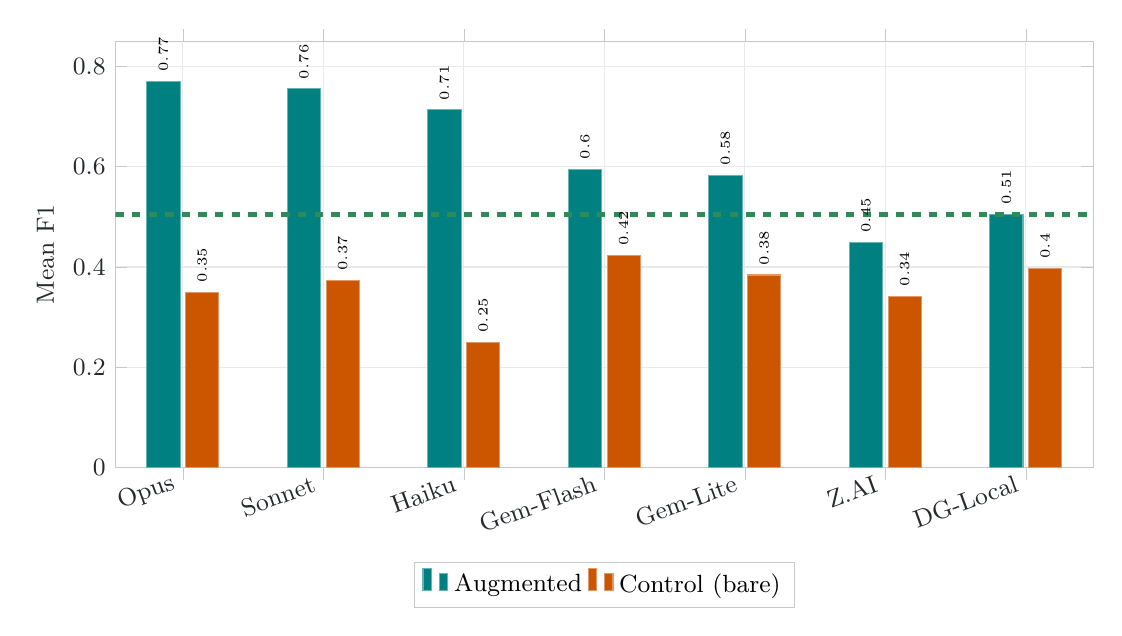
\begin{tikzpicture}
\begin{axis}[ybar,width=14cm,height=7cm,bar width=12pt,ymin=0,ymax=0.85,
  ylabel={Mean F1},
  symbolic x coords={Opus,Sonnet,Haiku,Gem-Flash,Gem-Lite,Z.AI,DG-Local},
  xtick=data,x tick label style={rotate=20,anchor=east,font=\small},
  enlarge x limits=0.08,
  legend style={at={(0.5,-0.22)},anchor=north,legend columns=3,draw=grayln},
  nodes near coords,nodes near coords style={font=\tiny,rotate=90,anchor=west}]
\addplot[augstyle] coordinates {(Opus,0.770) (Sonnet,0.755) (Haiku,0.713) (Gem-Flash,0.595) (Gem-Lite,0.583) (Z.AI,0.449) (DG-Local,0.505)};
\addplot[ctlstyle] coordinates {(Opus,0.350) (Sonnet,0.373) (Haiku,0.250) (Gem-Flash,0.423) (Gem-Lite,0.384) (Z.AI,0.342) (DG-Local,0.397)};
\draw[softgreen,line width=1.8pt,dashed] ({rel axis cs:0,0}|-{axis cs:Opus,0.505}) -- ({rel axis cs:1,0}|-{axis cs:Opus,0.505});
\legend{Augmented,Control (bare),DG+ontology line (0.505)}
\end{axis}\end{tikzpicture}
\caption{F1 by model. The dashed green line marks DiffusionGemma+ontology (0.505). Every frontier
model's \emph{bare} score falls below this line. Grounding lets a local 26B model outperform
cloud-hosted frontier models on domain-specific factual recall.}
\end{figure}

\begin{samepage}
\begin{table}[h]\centering\small
\begin{tabular}{lcccccc}
\toprule
Model & AUG F1 & CTL F1 & $\Delta$ & AUG Halluc & CTL Halluc & $\Delta$H \\
\midrule
Opus 4.8 & \textbf{0.770} & 0.350 & \textcolor{burnt}{+0.420} & 0.052 & 0.581 & \textcolor{teal0}{--0.529} \\
Sonnet 4.6 & 0.755 & 0.373 & \textcolor{burnt}{+0.382} & 0.079 & 0.559 & \textcolor{teal0}{--0.480} \\
Haiku 4.5 & 0.713 & 0.250 & \textcolor{burnt}{+0.463} & 0.106 & 0.714 & \textcolor{teal0}{--0.608} \\
Gemini 3.5 Flash & 0.595 & 0.423 & \textcolor{burnt}{+0.172} & 0.250 & 0.460 & \textcolor{teal0}{--0.210} \\
Gemini 2.5 Flash Lite & 0.583 & 0.384 & \textcolor{burnt}{+0.199} & 0.266 & 0.498 & \textcolor{teal0}{--0.232} \\
Z.AI (GLM-4.6) & 0.449 & 0.342 & \textcolor{burnt}{+0.108} & 0.188 & 0.394 & \textcolor{teal0}{--0.206} \\
\midrule
\textbf{DiffusionGemma (local)} & 0.505 & 0.397 & \textcolor{burnt}{+0.108} & 0.299 & 0.498 & \textcolor{teal0}{--0.199} \\
\bottomrule
\end{tabular}
\caption{Per-model results. All 7 models show positive augmentation delta and reduced
hallucination. Claude models show the largest absolute lift; DiffusionGemma's own lift is modest
but its grounded score exceeds every frontier bare score.}
\end{table}
\end{samepage}

% =============================================================================
% BY QUESTION TYPE
% =============================================================================
\section{Performance by Question Type}

\begin{samepage}
\begin{figure}[h]\centering
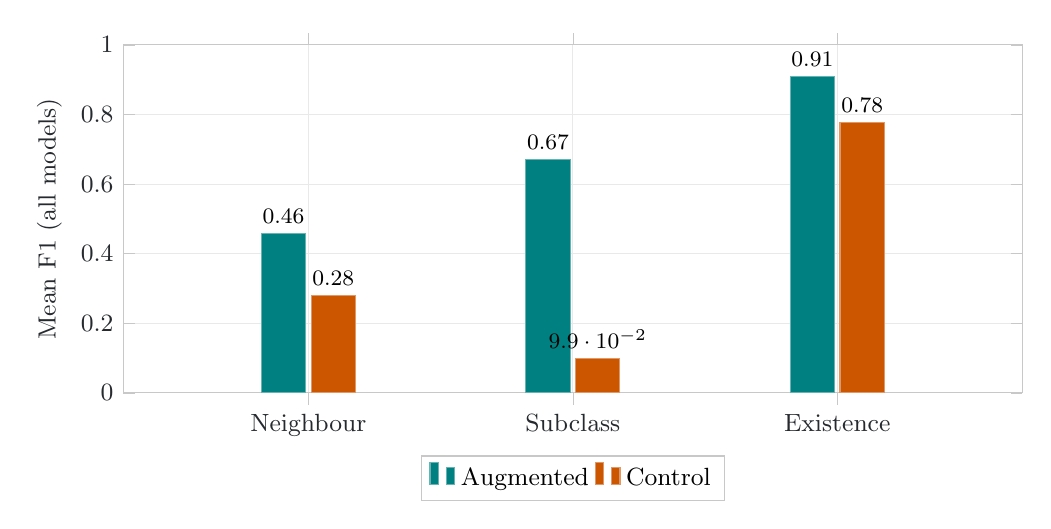
\begin{tikzpicture}
\begin{axis}[ybar,width=13cm,height=6cm,bar width=16pt,ymin=0,ymax=1,
  ylabel={Mean F1 (all models)},symbolic x coords={Neighbour,Subclass,Existence},xtick=data,
  enlarge x limits=0.35,legend style={at={(0.5,-0.18)},anchor=north,legend columns=2,draw=grayln},
  nodes near coords,nodes near coords style={font=\footnotesize}]
\addplot[augstyle] coordinates {(Neighbour,0.458) (Subclass,0.671) (Existence,0.910)};
\addplot[ctlstyle] coordinates {(Neighbour,0.281) (Subclass,0.099) (Existence,0.778)};
\legend{Augmented,Control}
\end{axis}\end{tikzpicture}
\caption{Subclass questions show the largest relative lift (+0.573 absolute). Existence questions
are easy for both arms (high baseline). Neighbour-recall benefits moderately.}
\end{figure}
\end{samepage}

\begin{samepage}
\begin{table}[h]\centering\small
\begin{tabular}{l*{6}{c}}
\toprule
 & \multicolumn{2}{c}{Neighbour} & \multicolumn{2}{c}{Subclass} & \multicolumn{2}{c}{Existence} \\
\cmidrule(lr){2-3}\cmidrule(lr){4-5}\cmidrule(lr){6-7}
Model & AUG & CTL & AUG & CTL & AUG & CTL \\
\midrule
Opus & 0.540 & 0.346 & 1.000 & 0.073 & 1.000 & 0.634 \\
Sonnet & 0.560 & 0.311 & 0.985 & 0.118 & 0.914 & 0.750 \\
Haiku & 0.551 & 0.208 & 0.750 & 0.188 & 1.000 & 0.396 \\
Gem-Flash & 0.440 & 0.311 & 0.500 & 0.071 & 1.000 & 1.000 \\
Gem-Lite & 0.434 & 0.232 & 0.464 & 0.071 & 1.000 & 1.000 \\
Z.AI & 0.357 & 0.312 & 0.500 & 0.075 & 0.583 & 0.667 \\
DG (local) & 0.323 & 0.248 & 0.500 & 0.094 & 0.875 & 1.000 \\
\bottomrule
\end{tabular}
\caption{Per-model $\times$ per-type F1. Claude models dominate subclass recall when grounded
(0.75--1.00); smaller models plateau at 0.50. DiffusionGemma's existence score is strong (0.875)
but neighbour recall is weak (0.323).}
\end{table}
\end{samepage}

% =============================================================================
% HALLUCINATION
% =============================================================================
\section{Hallucination Analysis}

\begin{samepage}
\begin{figure}[h]\centering
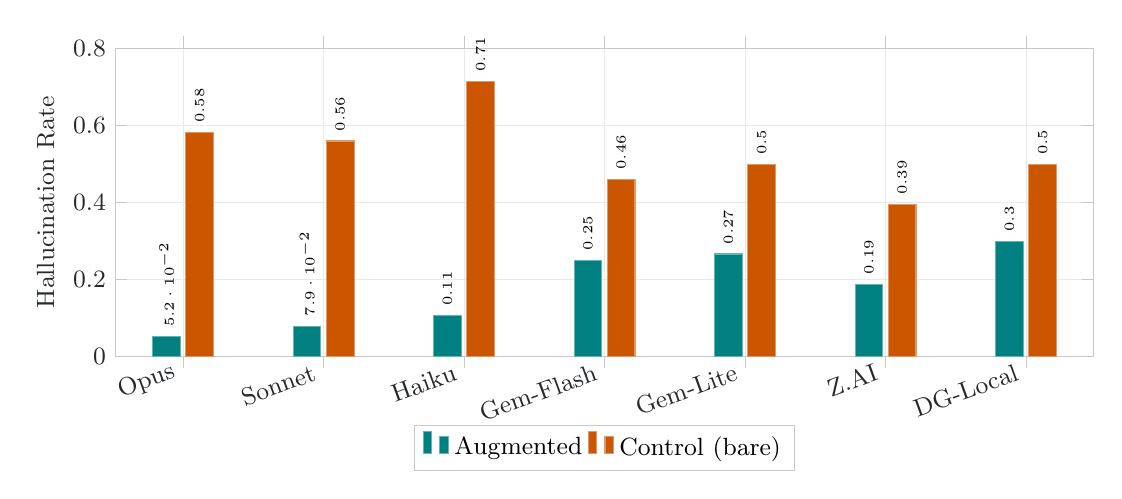
\begin{tikzpicture}
\begin{axis}[ybar,width=14cm,height=5.5cm,bar width=10pt,ymin=0,ymax=0.8,
  ylabel={Hallucination Rate},
  symbolic x coords={Opus,Sonnet,Haiku,Gem-Flash,Gem-Lite,Z.AI,DG-Local},
  xtick=data,x tick label style={rotate=20,anchor=east,font=\small},
  enlarge x limits=0.08,
  legend style={at={(0.5,-0.22)},anchor=north,legend columns=2,draw=grayln},
  nodes near coords,nodes near coords style={font=\tiny,rotate=90,anchor=west}]
\addplot[augstyle] coordinates {(Opus,0.052) (Sonnet,0.079) (Haiku,0.106) (Gem-Flash,0.250) (Gem-Lite,0.266) (Z.AI,0.188) (DG-Local,0.299)};
\addplot[ctlstyle] coordinates {(Opus,0.581) (Sonnet,0.559) (Haiku,0.714) (Gem-Flash,0.460) (Gem-Lite,0.498) (Z.AI,0.394) (DG-Local,0.498)};
\legend{Augmented,Control (bare)}
\end{axis}\end{tikzpicture}
\caption{Ontology grounding reduces hallucination for every model. The largest reduction is
Haiku (0.714\,$\to$\,0.106, --0.608). Even DiffusionGemma drops from 0.498 to 0.299.}
\end{figure}
\end{samepage}

% =============================================================================
% COST AND PRIVACY
% =============================================================================
\section{Cost, Privacy, and Inference Economics}

\begin{samepage}
\begin{table}[h]\centering\small
\begin{tabular}{lcccc}
\toprule
Model & F1 (best arm) & Data leaves org? & Per-query cost & Latency \\
\midrule
Opus 4.8 AUG & \textbf{0.770} & Yes (Anthropic API) & \$\,0.04--0.08 & 30--50\,s \\
Sonnet 4.6 AUG & 0.755 & Yes (Anthropic API) & \$\,0.01--0.02 & 15--30\,s \\
Haiku 4.5 AUG & 0.713 & Yes (Anthropic API) & \$\,0.002 & 8--15\,s \\
Gemini 3.5 Flash AUG & 0.595 & Yes (Google API) & \$\,0.003 & 5--10\,s \\
\midrule
\textbf{DG 26B AUG (local)} & \textbf{0.505} & \textbf{No} & \textbf{\$\,0\rlap{*}} & \textbf{2--4\,s} \\
\bottomrule
\end{tabular}
\caption{Cost and privacy comparison. DiffusionGemma runs entirely on-premise: no data leaves
the organisation, no per-query API cost, lowest latency. The ontology condense pass is a one-off
6-hour batch (7{,}445 classes), not per-query.\\
{\footnotesize *Amortised electricity/hardware only; no API billing.}}
\end{table}
\end{samepage}

Inference unit economics favour local deployment when query volume exceeds a few hundred
per day~\cite{introl2026inference}. For regulated industries where data must not leave the
organisation, GDPR-compliant on-premise inference is the only viable
path~\cite{advisori2026gdpr}. The ontology grounding cost is a one-time batch
($\sim$6\,h for 7{,}445 classes using DiffusionGemma locally); the per-query overhead is a
single read from the alias cache (sub-millisecond).

% =============================================================================
% CAVEATS
% =============================================================================
\section{Caveats on Lift Interpretation}
\label{sec:caveats}

The headline finding, that a local model with ontology grounding outperforms frontier models
without it, requires careful interpretation.

\begin{samepage}
\subsection{Grounded-local vs.\ bare-frontier: not like-for-like}
DiffusionGemma+ontology (0.505) beats Opus bare (0.350), but this is not an apples-to-apples
capability comparison. The local model receives structured KG triples as input context; the
frontier models receive only the question. If frontier models were also grounded, they would
score substantially higher: Opus AUG reaches 0.770, Sonnet AUG 0.755. The comparison
demonstrates the \emph{value of the ontology}, not the superiority of the local model's
reasoning.
\end{samepage}

\begin{samepage}
\subsection{Frontier models benefit far more from grounding}
The ontology amplifies capability rather than substituting for it. Claude models gain
+0.38--0.46 F1 from grounding; DiffusionGemma gains only +0.108. This asymmetry suggests that
larger models are better at \emph{exploiting} structured context: they extract more from the
same triples. The ontology is a capability multiplier, and the multiplier scales with the base.
\end{samepage}

\begin{samepage}
\subsection{DiffusionGemma's own augmentation lift is modest}
At +0.108 F1, the local model's lift is statistically meaningful but operationally small compared
to the frontier lifts. The primary driver of DiffusionGemma's competitive bare score (0.397) is
surprisingly strong parametric knowledge; it already knows many of the domain concepts. The
ontology's contribution to the local model is more about \emph{precision} (hallucination drops
from 0.498 to 0.299) than about \emph{recall}.
\end{samepage}

\begin{samepage}
\subsection{Performance varies sharply by question type}
DiffusionGemma+ontology excels on existence queries (0.875, near ceiling) and subclass queries
(0.500) but struggles on neighbour recall (0.323). The 256-token block decode window limits the
number of distinct class names the model can enumerate per response. Frontier models with longer
output windows (Opus neighbour AUG: 0.540) do not face this constraint. Headline F1 averages
over these disparate regimes; no single number captures the full picture.
\end{samepage}

\begin{samepage}
\subsection{Condense pass: a one-off cost}
We built the ontology alias index by running DiffusionGemma over all 7{,}445 OWL classes
($\sim$6 hours on a single GPU). This is amortised over all future queries, but it means the
system requires upfront investment. Re-indexing is needed when the KG changes materially.
\end{samepage}

\begin{samepage}
\subsection{Gold truth is the KG itself}
The evaluation measures fidelity to the knowledge graph's asserted ontology, not general-purpose
question answering. Results do not transfer directly to open-domain QA benchmarks. A model that
scores poorly here may still be excellent at tasks outside the KG's domain.
\end{samepage}

\begin{samepage}
\subsection{Sample size and domain scope}
16 questions $\times$ 3 reps $\times$ 7 models = 672 cells. While statistically powered for the
observed effect sizes (Cohen's $d > 1.0$ for Claude models), the question set is drawn from a
single domain (DreamLab's Web3/XR/AI ontology). Generalisation to other knowledge graphs and
domains is plausible but untested.
\end{samepage}

% =============================================================================
% FINDINGS
% =============================================================================
\section{Findings}
\begin{samepage}
\begin{enumerate}[leftmargin=1.3em]
\item \textbf{Ontology grounding is model-agnostic and universally beneficial.} All 7 models
      show positive F1 lift and reduced hallucination. The effect is strongest on niche,
      project-specific concepts where parametric knowledge is weakest.

\item \textbf{A local model + ontology can exceed frontier bare for domain-specific recall.}
      DiffusionGemma+ontology (0.505) beats every cloud model tested without grounding. This
      validates the thesis that structured retrieval compensates for raw parameter
      count~\cite{lewis2020rag,liu2024chatqa}.

\item \textbf{Grounding amplifies capability: frontier models gain the most.} Opus AUG (0.770)
      is the highest score observed. The ontology is a force multiplier, not an
      equaliser~(\S\ref{sec:caveats}).

\item \textbf{Subclass recall is the largest relative win.} From 0.099 (CTL) to 0.671 (AUG), a
      6.8$\times$ improvement. Models have almost no parametric knowledge of ontology hierarchies;
      the KG supplies it directly.

\item \textbf{Hallucination halves with grounding.} Overall 0.529 $\to$ 0.177, consistent with
      the KG-grounding literature~\cite{agrawal2023kghallucination,sansford2024kgtrustworthy}.

\item \textbf{Data sovereignty is achievable without sacrificing domain accuracy.}
      DiffusionGemma runs entirely on-premise with zero API cost. For regulated or
      privacy-sensitive deployments, this is the critical
      finding~\cite{advisori2026gdpr}.
\end{enumerate}
\end{samepage}

% =============================================================================
% THREATS
% =============================================================================
\section{Threats to Validity}
\begin{samepage}
\begin{itemize}[leftmargin=1.3em]
\item Gold is the KG's asserted graph; KG errors propagate to gold (mitigated by curating
      concepts with rich, sensible neighbourhoods).
\item The grader's token-set matching can over- or under-credit near-synonyms; thresholds were
      smoke-validated for non-saturation before the full run.
\item The augmented arm uses the skill CLI, not the MCP tool directly; both share the same
      \texttt{createDefaultRetrieval} brain, so results transfer.
\item DiffusionGemma's 256-token block decode constrains neighbour enumeration; autoregressive
      models do not face this limit. A fairer neighbour comparison would cap output tokens.
\item Gemini and Z.AI models were accessed via their respective commercial APIs; rate limits and
      non-determinism at temperature=0 may introduce variance not present in locally-hosted models.
\end{itemize}
\end{samepage}

\printbibliography[title={References}]

\end{document}
